%versi 3 (22-07-2020)
\chapter{Landasan Teori}
\label{chap:teori}

\section{Hypertext Markup Language (HTML)}
\label{sec:html}
\subsection{Pengertian HTML}
 
\textit{Hypertext Markup Language} (HTML) merupakan bahasa markup yang digunakan untuk menyusun struktur dasar halaman web. HTML tidak termasuk bahasa pemrograman karena tidak memiliki mekanisme logika seperti percabangan, perulangan, atau pengolahan data secara langsung, melainkan digunakan untuk mendeskripsikan struktur dan makna konten yang akan ditampilkan pada browser~\cite{duckett:11:htmlcss}. HTML memungkinkan pengembang mengatur berbagai jenis konten, seperti teks, gambar, tautan, tabel, formulir, serta elemen multimedia lainnya dalam sebuah dokumen web.

HTML berfungsi sebagai kerangka utama halaman web yang menentukan bagaimana setiap bagian konten disusun sehingga dapat ditampilkan secara terstruktur oleh browser~\cite{duckett:11:htmlcss}. Dalam pengembangan web, HTML umumnya digunakan bersama dengan CSS dan JavaScript. HTML berperan dalam membentuk struktur konten, CSS digunakan untuk mengatur tampilan atau gaya visual, sedangkan JavaScript digunakan untuk menambahkan interaktivitas pada halaman web.

HTML bekerja dengan konsep \textit{tag-based structure}, yaitu setiap elemen ditandai dengan tag tertentu. Tag tersebut memberikan informasi kepada browser mengenai jenis dan fungsi konten, misalnya paragraf, judul, gambar, tautan, atau daftar. Melalui struktur ini, browser dapat memahami peran masing-masing elemen, menyusun hubungan antar elemen, dan menampilkannya dengan benar kepada pengguna.

\subsection{Elemen dan Tag HTML}
Elemen HTML merupakan komponen dasar dalam penyusunan halaman web. Setiap elemen digunakan untuk merepresentasikan bagian tertentu dari konten, seperti paragraf, judul, gambar, tautan, tabel, daftar, maupun formulir. Secara umum, sebuah elemen HTML terdiri dari tag pembuka, isi elemen, dan tag penutup. Sebagai contoh, elemen paragraf dituliskan dengan <p> sebagai tag pembuka, isi teks sebagai konten, dan </p> sebagai tag penutup.

Tag berfungsi sebagai penanda yang memberi tahu browser mengenai jenis elemen yang sedang digunakan. Tag pembuka menunjukkan awal suatu elemen, sedangkan tag penutup menunjukkan akhir elemen tersebut. Namun, tidak semua elemen HTML memiliki tag penutup. Beberapa elemen, seperti <img>, <br>, dan <hr>, termasuk elemen kosong karena tidak memiliki isi di antara tag pembuka dan tag penutup.

Selain tag, elemen HTML juga dapat memiliki atribut yang memberikan informasi tambahan terhadap elemen tersebut. Atribut dituliskan di dalam tag pembuka dan umumnya terdiri dari nama atribut serta nilai atribut. Sebagai contoh, atribut href pada elemen <a> digunakan untuk menentukan alamat tautan, sedangkan atribut src pada elemen <img> digunakan untuk menentukan lokasi berkas gambar. Atribut lain seperti id dan class sering digunakan untuk memberi identitas atau pengelompokan elemen agar dapat diatur lebih lanjut menggunakan CSS atau diproses melalui JavaScript.

Struktur elemen yang saling bersarang ({\it nested elements}) memungkinkan terbentuknya hubungan hierarkis antar elemen. Dalam struktur ini, suatu elemen dapat menjadi induk bagi elemen lain yang berada di dalamnya. Misalnya, elemen <body> dapat memuat elemen <div>, kemudian elemen <div> tersebut dapat memuat elemen <p>, <img>, atau <a>. Hubungan bertingkat ini menjadi dasar penting dalam pembentukan struktur DOM karena browser akan membaca dokumen HTML sebagai susunan node yang saling terhubung.

\begin{figure} [H]
	\centering  
	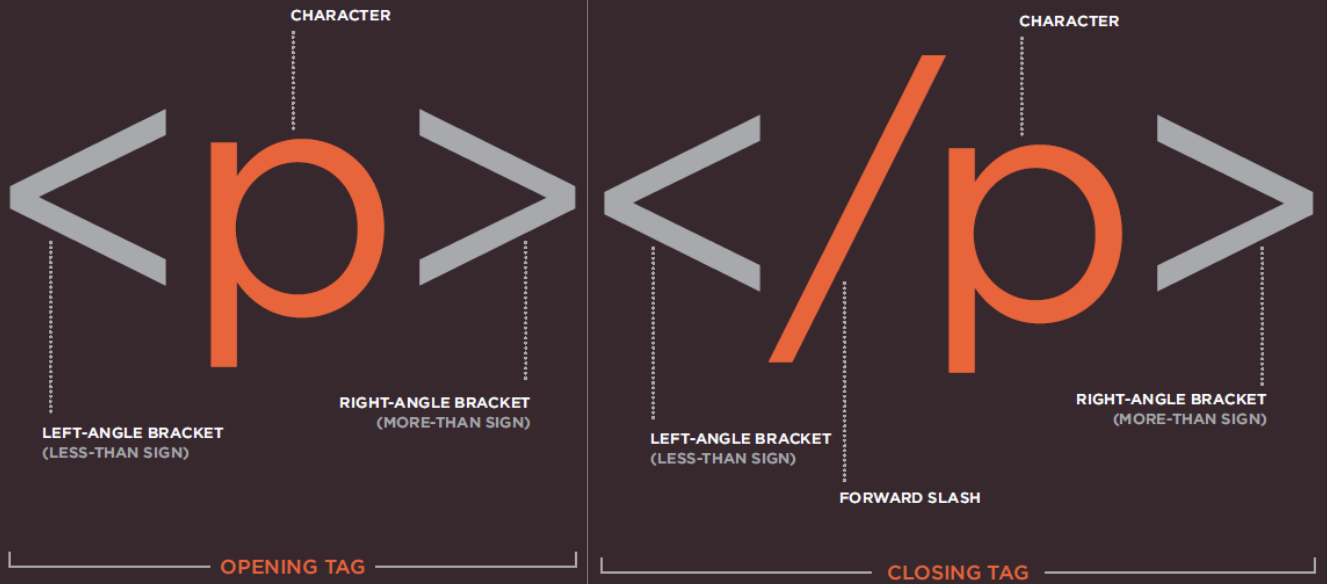
\includegraphics[scale=0.3]{../Gambar/TagHTML.png}
	\caption[Gambar Tag pembuka dan penutup]{Contoh tag pembuka dan penutup dokumen HTML} 
	\label{fig:htmlpng} 
\end{figure}

%\dtext{11-12} 

\subsection{Struktur dasar HTML}
\label{sec:struktur}
Dokumen HTML memiliki struktur standar yang terdiri dari beberapa bagian utama, yaitu <html>, <head>, dan <body>. Struktur tersebut biasanya diawali dengan deklarasi <!DOCTYPE html> yang berfungsi untuk memberi tahu browser bahwa dokumen menggunakan standar HTML modern. Setelah deklarasi tersebut, elemen <html> digunakan sebagai root dari seluruh dokumen HTML dan menjadi wadah bagi elemen-elemen lain di dalam halaman web.

Elemen <head> berisi informasi yang tidak ditampilkan secara langsung pada halaman, tetapi dibutuhkan oleh browser dan mesin pencari untuk memahami dokumen. Informasi tersebut dapat berupa judul halaman melalui elemen <title>, pengaturan karakter melalui elemen <meta>, pemanggilan berkas CSS melalui elemen <link>, serta pemanggilan skrip tertentu melalui elemen <script>. Bagian ini berperan penting dalam pengaturan metadata, optimasi halaman, dan hubungan dokumen HTML dengan sumber daya eksternal.

Elemen <body> berisi seluruh konten utama yang ditampilkan kepada pengguna pada browser. Konten tersebut dapat berupa teks, gambar, tautan, tabel, formulir, daftar, maupun elemen multimedia. Dengan demikian, bagian <body> menjadi tempat penyusunan tampilan utama halaman web yang dapat dilihat dan berinteraksi langsung dengan pengguna.

Struktur dasar ini memastikan bahwa setiap halaman web memiliki susunan yang konsisten dan dapat dipahami oleh browser. Ketika sebuah dokumen HTML dimuat, browser akan membaca struktur tersebut dari bagian paling atas, memproses metadata pada <head>, kemudian menampilkan konten yang terdapat pada <body>. Susunan yang teratur juga memudahkan proses pembentukan DOM karena setiap elemen memiliki posisi dan hubungan yang jelas di dalam hierarki dokumen.

\begin{figure} [H]
	\centering  
	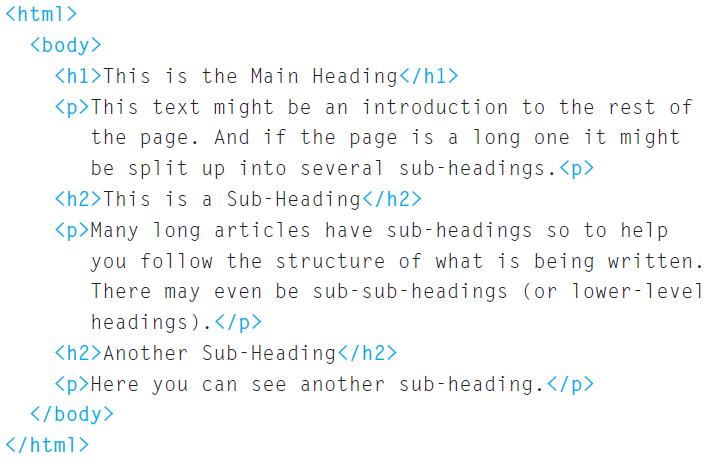
\includegraphics[scale=0.5]{../Gambar/StrukturDasarHTML2.png}
	\caption[Gambar Struktur dasar HTML]{Contoh struktur dasar dokumen HTML} 
	\label{fig:strukturdasarhtml} 
\end{figure}

\subsection{Hierarki elemen HTML}

Struktur HTML bersifat hierarkis, yang berarti elemen dapat berada di dalam elemen lain. Hubungan antar elemen ini membentuk struktur bertingkat yang menyerupai pohon, di mana setiap elemen memiliki posisi tertentu dalam dokumen. Dalam struktur tersebut, elemen yang memuat elemen lain disebut sebagai parent, sedangkan elemen yang berada di dalamnya disebut sebagai child. Elemen-elemen yang berada pada tingkat yang sama dan memiliki parent yang sama disebut sebagai sibling.

Sebagai contoh, elemen <body> dapat berperan sebagai parent bagi elemen <div>. Selanjutnya, elemen <div> dapat berisi elemen <p>, <img>, atau <a> sebagai child. Jika di dalam satu elemen <div> terdapat beberapa elemen <p>, maka elemen-elemen tersebut dapat disebut sebagai sibling karena berada pada tingkat hierarki yang sama. Hubungan seperti ini menunjukkan bahwa dokumen HTML tidak hanya tersusun secara berurutan, tetapi juga memiliki hubungan induk-anak yang jelas antar elemen.

Hierarki ini penting karena menentukan bagaimana elemen saling berhubungan dan bagaimana struktur tersebut akan diproses menjadi DOM. Ketika browser membaca dokumen HTML, setiap elemen akan direpresentasikan sebagai node dalam struktur DOM. Hubungan parent, child, dan sibling pada HTML akan menjadi dasar pembentukan hubungan antar node di dalam DOM. Oleh karena itu, susunan elemen yang benar akan memudahkan browser dalam memahami struktur dokumen dan menampilkan halaman web secara sesuai.

Semakin kompleks halaman web, maka semakin dalam dan luas struktur hierarki yang terbentuk. Halaman yang memiliki banyak bagian, seperti header, navigasi, konten utama, sidebar, formulir, dan footer, akan menghasilkan struktur HTML yang lebih bercabang. Struktur hierarkis tersebut juga memengaruhi proses penelusuran elemen, baik dalam manipulasi DOM menggunakan JavaScript maupun dalam analisis struktur halaman menggunakan pendekatan traversal seperti DFS.

%\dtext{13-14}


\section{Document Object Model (DOM)}
\label{sec:dom}

 \subsection{Pengertian DOM}
\textit{Document Object Model }(DOM) adalah representasi dari dokumen HTML dalam bentuk struktur objek yang dapat diakses dan dimanipulasi oleh program. DOM memungkinkan setiap elemen dalam halaman web diperlakukan sebagai objek yang memiliki properti dan metode~\cite{marini:02:thedom}.

Menurut \textit{World Wide Web Consortium}, DOM menyediakan antarmuka standar untuk mengakses dan memodifikasi dokumen HTML.

Dengan adanya DOM, halaman web tidak hanya menjadi tampilan statis, tetapi juga dapat diproses dan dimodifikasi secara dinamis.

\subsection{Struktur DOM sebagai Tree}
Struktur DOM berbentuk pohon (tree structure), di mana setiap elemen HTML direpresentasikan sebagai node. Node paling atas disebut root node, yang biasanya adalah elemen <html>.
Setiap node dapat memiliki:
\begin{itemize}
    \item Parent (induk)
    \item Child (anak)
    \item Sibling (saudara) 
\end{itemize}
Struktur ini memungkinkan proses traversal dilakukan secara sistematis, seperti menggunakan DFS.

\subsection{Jenis node pada DOM}
DOM terdiri dari beberapa jenis node, antara lain:
\begin{itemize}
    \item Element node: merepresentasikan tag HTML
    \item Text node: merepresentasikan isi teks
    \item Attribute node: merepresentasikan atribut 
\end{itemize}
Keberadaan berbagai jenis node ini membuat struktur DOM lebih kompleks dibandingkan HTML mentah, sehingga analisis DOM memberikan informasi yang lebih lengkap.
 
%\dtext{15-16}

\section{Parsing HTML}
\subsection{Pengertian Parsing HTML}
Parsing HTML adalah proses membaca dan menganalisis dokumen HTML untuk membentuk struktur yang dapat dipahami dan diproses oleh program. Pada proses ini, teks HTML yang tersusun dari tag, atribut, dan konten akan diinterpretasikan menjadi struktur yang lebih terorganisasi. Browser melakukan proses parsing untuk memahami susunan dokumen HTML sebelum membentuk DOM dan menampilkan halaman web kepada pengguna.

Dalam konteks pengolahan dokumen web, parsing HTML penting karena dokumen HTML tidak hanya berisi teks biasa, tetapi juga memiliki struktur tag yang saling bersarang. Melalui proses parsing, setiap elemen dapat dikenali berdasarkan tag, atribut, posisi, dan hubungannya dengan elemen lain. Hasil parsing inilah yang kemudian dapat digunakan untuk analisis struktur halaman, ekstraksi informasi, maupun pembentukan representasi DOM.

\subsection{Hubungan Parsing HTML dengan DOM}
Parsing HTML memiliki hubungan erat dengan pembentukan DOM. Ketika sebuah dokumen HTML diproses, parser akan membaca elemen-elemen HTML secara berurutan dan membentuk struktur node yang merepresentasikan dokumen tersebut. Struktur node ini kemudian menjadi DOM tree, yaitu representasi hierarkis dari dokumen HTML.

Pada penelitian ini, proses parsing HTML menjadi tahap awal yang penting sebelum struktur DOM direpresentasikan sebagai graf. Elemen-elemen hasil parsing dapat dipetakan menjadi node, sedangkan hubungan antar elemen seperti parent dan child dapat dipetakan menjadi edge. Dengan demikian, parsing HTML menjadi penghubung antara dokumen HTML mentah dan struktur graf yang dapat dianalisis serta divisualisasikan.

\section{Struktur Data Tree}
\subsection{Pengertian Tree}
Tree adalah struktur data hierarkis yang terdiri dari sekumpulan node dan hubungan antar node. Node paling atas dalam tree disebut root, sedangkan node yang berada di bawah node lain disebut child. Node yang memiliki child disebut parent, sementara node yang tidak memiliki child disebut leaf. Struktur tree digunakan untuk merepresentasikan hubungan bertingkat, yaitu satu node dapat memiliki beberapa node turunan.

Secara konsep, tree merupakan bentuk khusus dari graf yang tidak memiliki siklus dan memiliki hubungan hierarkis yang jelas. Setiap node dalam tree, kecuali root, memiliki satu parent. Karakteristik ini membuat tree cocok digunakan untuk memodelkan struktur yang tersusun secara bertingkat, seperti struktur folder, organisasi data, ekspresi matematika, dan dokumen HTML.

\subsection{Tree pada Struktur DOM}
DOM memiliki karakteristik yang menyerupai tree karena setiap elemen dalam dokumen HTML tersusun secara hierarkis. Elemen <html> biasanya menjadi root, sedangkan elemen <head> dan <body> menjadi child dari elemen tersebut. Selanjutnya, elemen-elemen lain seperti <div>, <p>, <img>, dan <a> dapat menjadi turunan dari elemen <body> atau elemen lain di dalamnya.

Pemahaman mengenai tree penting dalam penelitian ini karena struktur DOM yang berbentuk tree dapat ditelusuri menggunakan algoritma traversal. Salah satu algoritma yang sesuai untuk struktur seperti ini adalah DFS, karena DFS menelusuri node secara mendalam dari root menuju leaf sebelum kembali ke cabang lain. Dengan demikian, konsep tree menjadi dasar untuk memahami hubungan antara DOM, graf, dan proses traversal.

\section{Struktur Data Graf}
\subsection{Pengertian Graf}
Graf adalah struktur data yang terdiri dari simpul ({\it node} atau {\it vertex}) dan sisi ({\it edge}) yang menghubungkan simpul-simpul tersebut. Dalam kajian algoritma, graf umumnya dinyatakan sebagai pasangan himpunan $G=(V,E)$, dengan $V$ sebagai himpunan simpul dan $E$ sebagai himpunan sisi yang merepresentasikan hubungan antar simpul~\cite{cormen:22:introalgo}. Setiap simpul dapat menggambarkan suatu objek, sedangkan sisi menunjukkan adanya relasi atau keterhubungan antara dua objek.

Menurut Cormen, graf banyak digunakan untuk memodelkan berbagai jenis hubungan dalam komputasi karena bentuknya fleksibel dan dapat merepresentasikan struktur yang sederhana maupun kompleks~\cite{cormen:22:introalgo}. Sebagai contoh, simpul dapat merepresentasikan kota, halaman web, pengguna, proses, atau elemen dalam dokumen, sedangkan sisi dapat merepresentasikan jalan, tautan, hubungan sosial, komunikasi antar proses, atau hubungan induk-anak antar elemen.

Graf dapat dibedakan berdasarkan karakteristik sisinya. Pada graf tidak berarah, hubungan antar simpul tidak memiliki arah tertentu sehingga relasi antara dua simpul dianggap berlaku dua arah. Sebaliknya, pada graf berarah, setiap sisi memiliki arah dari satu simpul ke simpul lainnya. Selain itu, graf juga dapat memiliki bobot pada sisi untuk menyatakan nilai tertentu, seperti jarak, biaya, waktu, atau tingkat hubungan antar simpul.

Dalam konteks penelitian ini, konsep graf digunakan untuk merepresentasikan struktur DOM dari dokumen HTML. Setiap elemen HTML dapat dipandang sebagai simpul, sedangkan hubungan antara elemen induk dan elemen anak dapat dipandang sebagai sisi. Dengan pemodelan tersebut, struktur halaman web dapat dianalisis menggunakan konsep teori graf, seperti hubungan antar node, arah hubungan, dan proses traversal.

\subsection{Representasi Graf}
Representasi graf adalah cara menyimpan struktur graf agar dapat diproses oleh komputer. Dalam implementasi algoritma, graf tidak cukup hanya didefinisikan sebagai himpunan simpul dan sisi, tetapi perlu direpresentasikan dalam bentuk data tertentu. Dua bentuk representasi graf yang umum digunakan adalah adjacency matrix dan adjacency list~\cite{cormen:22:introalgo}.

Adjacency matrix merepresentasikan graf dalam bentuk matriks dua dimensi. Setiap baris dan kolom mewakili simpul, sedangkan nilai pada sel matriks menunjukkan ada atau tidaknya sisi antara dua simpul. Representasi ini mudah dipahami dan efisien untuk memeriksa hubungan langsung antar simpul, tetapi dapat menggunakan ruang penyimpanan yang besar jika jumlah simpul banyak dan jumlah sisi sedikit.

Adjacency list merepresentasikan graf dengan menyimpan daftar tetangga untuk setiap simpul. Setiap simpul memiliki daftar node lain yang terhubung dengannya. Representasi ini lebih hemat ruang untuk graf yang memiliki jumlah sisi relatif sedikit dibandingkan jumlah kemungkinan sisi. Dalam konteks DOM, adjacency list sesuai digunakan karena setiap elemen biasanya hanya memiliki hubungan langsung dengan sejumlah child tertentu, bukan dengan seluruh elemen dalam dokumen.

\subsection{Graf Berarah}
Graf berarah ({\it directed graph} atau {\it digraph}) adalah graf yang setiap sisinya memiliki arah tertentu. Pada graf berarah, sisi tidak hanya menunjukkan bahwa dua simpul saling terhubung, tetapi juga menunjukkan arah hubungan dari satu simpul menuju simpul lainnya. Secara formal, sisi pada graf berarah dapat dinyatakan sebagai pasangan terurut $(u,v)$, yang berarti sisi tersebut berawal dari simpul $u$ dan menuju simpul $v$~\cite{cormen:22:introalgo}.

Berbeda dengan graf tidak berarah, hubungan pada graf berarah tidak selalu berlaku dua arah. Jika terdapat sisi dari simpul $u$ ke simpul $v$, maka hal tersebut tidak secara otomatis berarti terdapat sisi dari simpul $v$ ke simpul $u$. Oleh karena itu, arah sisi menjadi informasi penting dalam memahami pola hubungan antar simpul. Konsep ini banyak digunakan untuk memodelkan hubungan yang memiliki alur, urutan, atau ketergantungan, seperti tautan antar halaman web, aliran data, proses kerja, maupun struktur hierarkis.

Dalam konteks DOM, hubungan antara parent dan child memiliki arah yang jelas, yaitu dari node induk menuju node anak. Misalnya, elemen <html> memiliki hubungan ke elemen <head> dan <body>, kemudian elemen <body> dapat memiliki hubungan ke elemen <div>, <p>, atau elemen lainnya. Arah hubungan tersebut menunjukkan bahwa suatu elemen berada di bawah elemen lain dalam struktur dokumen.

Pemodelan DOM sebagai graf berarah membantu menunjukkan alur hubungan antar elemen secara lebih terstruktur. Dengan menggunakan arah sisi, proses penelusuran dapat dilakukan dari root node menuju node-node turunannya. Hal ini penting dalam analisis struktur halaman web karena urutan dan arah hubungan antar elemen memengaruhi cara DOM dibaca, divisualisasikan, dan ditelusuri menggunakan algoritma traversal seperti DFS.

\begin{figure} [H]
	\centering  
	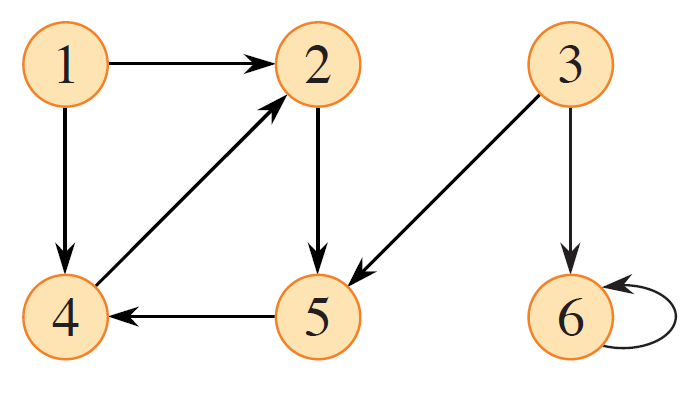
\includegraphics[scale=0.65]{../Gambar/digraph2.png}
	\caption[Contoh graf berarah sederhana (node dan edge)]{Contoh graf berarah sederhana (node dan edge)} 
	\label{fig:digraph} 
\end{figure}

\subsection{Representasi DOM sebagai graf}
Struktur DOM dapat direpresentasikan sebagai graf dengan cara memetakan setiap elemen HTML sebagai node dan hubungan parent-child sebagai edge. Dalam representasi ini, elemen root seperti <html> menjadi node awal, sedangkan elemen-elemen turunannya seperti <head>, <body>, <div>, <p>, dan elemen lain menjadi node yang terhubung melalui edge.

Karena hubungan antar elemen dalam DOM memiliki arah dari parent menuju child, struktur DOM lebih sesuai dimodelkan sebagai graf berarah. Setiap edge menunjukkan hubungan hierarkis antara dua elemen. Misalnya, hubungan dari <body> ke <div> menunjukkan bahwa elemen <div> berada di dalam elemen <body>. Dengan pemetaan ini, struktur HTML yang semula berbentuk dokumen teks dapat dianalisis sebagai struktur node dan edge.

Representasi DOM sebagai graf mempermudah proses analisis dan visualisasi struktur halaman web. Melalui pendekatan graf, hubungan antar elemen dapat ditelusuri menggunakan algoritma traversal seperti DFS. Selain itu, representasi ini juga mempermudah pembuatan visualisasi menggunakan Graphviz karena struktur DOM dapat diubah ke dalam format DOT dan ditampilkan sebagai diagram graf.

\subsection{Pengertian Traversal Graf}
Traversal graf adalah proses mengunjungi setiap node dalam graf secara sistematis berdasarkan aturan tertentu. Proses ini dilakukan untuk menelusuri hubungan antar node sehingga seluruh struktur graf dapat diproses tanpa ada node yang terlewat. Dalam kajian algoritma, traversal menjadi langkah penting karena banyak permasalahan graf membutuhkan proses pemeriksaan node dan edge, misalnya untuk mencari jalur, menentukan keterhubungan, menemukan komponen, atau menganalisis struktur hubungan antar objek~\cite{cormen:22:introalgo}.

Pada proses traversal, suatu node biasanya dipilih sebagai titik awal, kemudian algoritma akan menelusuri node-node lain yang terhubung melalui edge. Urutan kunjungan node bergantung pada metode traversal yang digunakan. Beberapa metode traversal yang umum digunakan adalah {\it Breadth-First Search} (BFS) dan {\it Depth-First Search} (DFS). BFS menelusuri node berdasarkan tingkat kedekatan dari node awal, sedangkan DFS menelusuri node secara mendalam hingga mencapai cabang terdalam sebelum kembali ke node sebelumnya.

Dalam konteks penelitian ini, traversal graf digunakan untuk menelusuri struktur DOM yang telah direpresentasikan sebagai graf. Setiap elemen HTML dipandang sebagai node, sedangkan hubungan parent-child dipandang sebagai edge. Dengan traversal, struktur halaman web dapat dibaca secara teratur dari node awal menuju node-node turunannya. Hal ini membantu proses analisis DOM karena setiap elemen dapat diperiksa sesuai urutan hubungan hierarkisnya.

\subsection{Depth-First Search}
{\it Depth-First Search} (DFS) adalah metode traversal graf yang bekerja dengan menelusuri suatu simpul hingga ke bagian terdalam terlebih dahulu sebelum kembali ke simpul sebelumnya. Sesuai dengan namanya, DFS akan memilih untuk bergerak lebih dalam pada graf selama masih terdapat sisi yang belum dieksplorasi dari simpul yang sedang dikunjungi.

Menurut Cormen, DFS mengeksplorasi sisi-sisi yang keluar dari simpul yang paling baru ditemukan dan masih memiliki sisi yang belum diperiksa. Jika seluruh sisi dari simpul tersebut telah dieksplorasi, proses pencarian akan melakukan {\it backtracking}, yaitu kembali ke simpul asal tempat simpul tersebut ditemukan untuk melanjutkan eksplorasi sisi lain yang belum dikunjungi~\cite{cormen:22:introalgo}. Proses ini berlanjut hingga seluruh simpul yang dapat dicapai dari simpul awal berhasil ditemukan. Apabila masih terdapat simpul lain yang belum ditemukan, DFS akan memilih simpul tersebut sebagai sumber baru dan mengulangi proses pencarian sampai seluruh simpul dalam graf telah diperiksa.

Dalam prosesnya, DFS juga mencatat hubungan pendahulu ({\it predecessor}) dari setiap simpul yang ditemukan. Ketika suatu simpul baru ditemukan dari simpul lain, hubungan tersebut dicatat sebagai bagian dari struktur hasil pencarian. Pada graf yang tidak seluruh simpulnya terhubung dari satu sumber, DFS dapat menghasilkan beberapa pohon pencarian, sehingga hasil keseluruhannya disebut sebagai {\it depth-first forest}. Sisi-sisi yang membentuk hubungan pendahulu tersebut dikenal sebagai {\it tree edges}~\cite{cormen:22:introalgo}.

DFS menggunakan penandaan warna untuk menunjukkan status setiap simpul selama proses traversal. Simpul yang belum dikunjungi diberi warna putih, simpul yang sedang diproses diberi warna abu-abu, dan simpul yang seluruh sisi keluarnya telah selesai diperiksa diberi warna hitam. Selain itu, DFS juga mencatat dua waktu pada setiap simpul, yaitu waktu penemuan ({\it discovery time}) ketika simpul pertama kali dikunjungi dan waktu penyelesaian ({\it finishing time}) ketika seluruh daftar ketetanggaan simpul tersebut telah selesai diperiksa. Informasi ini berguna untuk memahami urutan traversal dan struktur hubungan antar simpul dalam graf~\cite{cormen:22:introalgo}.

Metode ini sangat cocok untuk struktur berbentuk tree seperti DOM karena mengikuti pola parent-child secara mendalam. Pada konteks DOM, DFS dapat digunakan untuk menelusuri elemen dari node induk ke node anak secara bertahap hingga mencapai elemen terdalam, kemudian kembali ke node sebelumnya untuk melanjutkan penelusuran ke cabang lain. Oleh karena itu, DFS sering digunakan untuk eksplorasi struktur hierarkis dan graf~\cite{cormen:22:introalgo}.

\begin{figure} [H]
	\centering  
	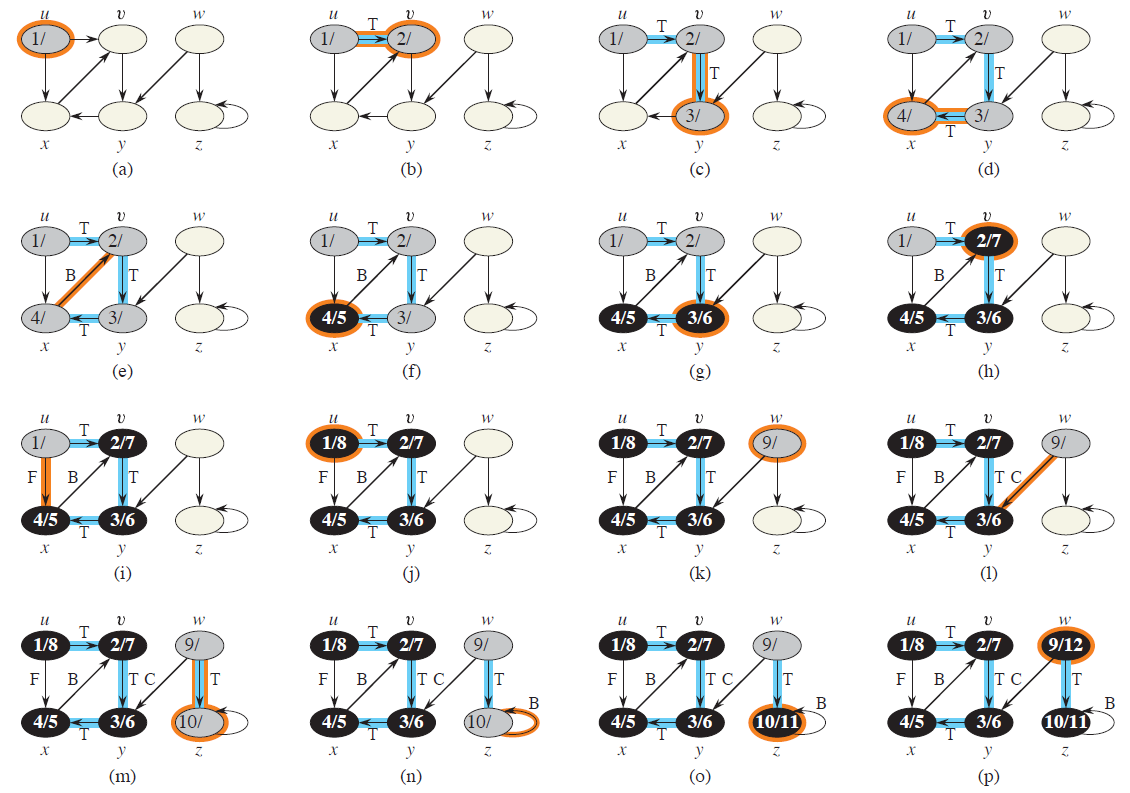
\includegraphics[scale=0.65]{../Gambar/DFS.png}
	\caption[Ilustrasi proses DFS pada Graf berarah]{Ilustrasi proses DFS pada graf berarah. Sisi-sisi diklasifikasikan sesuai urutan penjelajahannya: sisi pohon diberi label T, sisi belakang B, sisi depan F, dan sisi silang C.} 
	\label{fig:dfs} 
\end{figure}

\section{Graphviz}
\subsection{Pengertian Graphviz}
Graphviz adalah perangkat lunak visualisasi grafik \textit{open source}. Visualisasi grafik adalah cara untuk merepresentasikan informasi struktural sebagai diagram grafik abstrak dan jaringan. Teknologi ini memiliki aplikasi penting dalam jaringan, bioinformatika, rekayasa perangkat lunak, desain basis data dan web, pembelajaran mesin, dan antarmuka visual untuk domain teknis lainnya\cite{ellson:24:graphviz}.

Menurut \textit{Graphviz Project}, Graphviz menyediakan berbagai algoritma layout untuk menampilkan graf secara otomatis.

\subsection{Format DOT}
Graphviz menggunakan format DOT untuk mendefinisikan graf. DOT merupakan bahasa deskripsi graf berbasis teks yang digunakan untuk menuliskan struktur node dan edge secara sederhana. Melalui format ini, pengguna dapat menentukan jenis graf, nama graf, hubungan antar node, serta atribut visual seperti label, warna, bentuk node, dan arah hubungan. Graf tidak berarah pada DOT didefinisikan menggunakan kata kunci {\it graph} dengan simbol --, sedangkan graf berarah didefinisikan menggunakan kata kunci {\it digraph} dengan simbol ->.

Format DOT sesuai digunakan untuk merepresentasikan struktur DOM karena hubungan antar elemen HTML bersifat hierarkis dan berarah dari parent menuju child. Misalnya, hubungan antara elemen HTML dan head dapat dituliskan sebagai HTML -> head, yang menunjukkan adanya edge dari node HTML menuju node head. Dalam konteks penelitian ini, DOT digunakan sebagai format perantara untuk mengubah struktur DOM menjadi representasi graf yang kemudian dapat divisualisasikan menggunakan Graphviz.

\begin{figure} [H]
	\centering  
	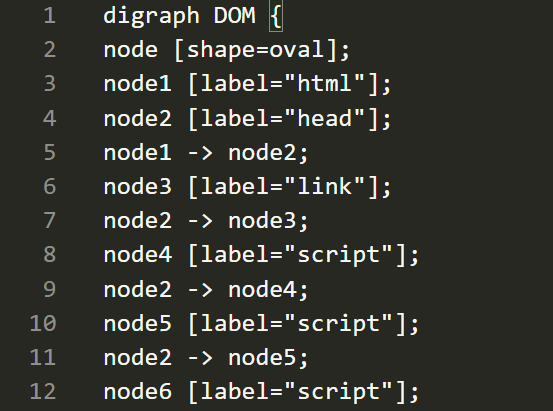
\includegraphics[scale=0.65]{../Gambar/DOT.png}
	\caption[Potongan Kode dengan format DOT]{Potongan kode .dot menggambarkan struktur DOM sederhana di mana HTML terhubung ke head, dan head memiliki beberapa elemen anak seperti link dan script} 
	\label{fig:dot} 
\end{figure}

\begin{figure} [H]
	\centering  
	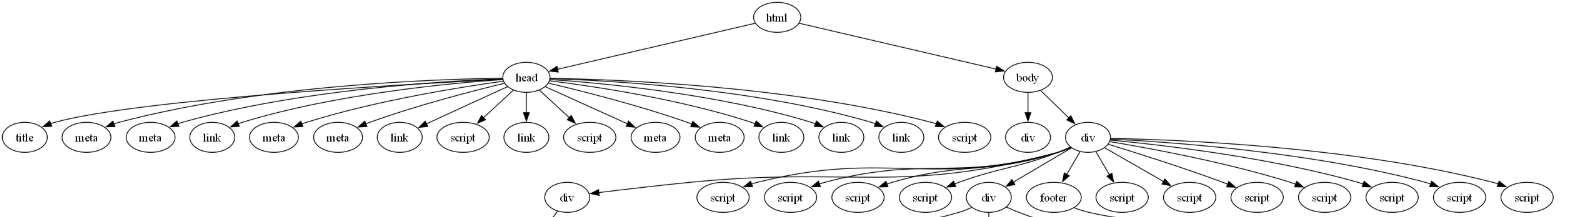
\includegraphics[scale=0.55]{../Gambar/VisualisasiDOM.png}
	\caption[Visualisasi dari format DOT dengan menggunakan Graphviz]{Visualisasi dari format DOT dengan menggunakan Graphviz} 
	\label{fig:visdot} 
\end{figure}

%\subsection{Tabel}  
%Berikut adalah contoh pembuatan tabel. 
%Penempatan tabel dan gambar secara umum diatur secara otomatis oleh \LaTeX{}, perhatikan contoh di file bab2.tex untuk melihat bagaimana cara memaksa tabel ditempatkan sesuai keinginan kita.

%Perhatikan bawa berbeda dengan penempatan judul gambar gambar, keterangan tabel harus diletakkan di atas tabel!!
%Lihat Tabel~\ref{tab:contoh1} berikut ini:

%\begin{table}[H] %atau h saja untuk "kira kira di sini"
	%\centering 
	%\caption{Tabel contoh}
	%\label{tab:contoh1}
	%\begin{tabular}{cccc}
		%\toprule
		%& $v_{start}$ & $\mathcal{S}_{1}$ & $v_{end}$\\

		%\midrule
		%$\tau_{1}$ & 1 & 12& 20\\
		%$\tau_{2}$ & 1 &  & 20\\
		%$\tau_{3}$ & 1 & 9 & 20\\
		%$\tau_{4}$ & 1 &  & 20\\

		%\bottomrule
		
	%\end{tabular} 
%\end{table}
%Tabel~\ref{tab:cthwarna1} dan Tabel~\ref{tab:cthwarna2} berikut ini adalah tabel dengan sel yang berwarna dan ada dua tabel yang bersebelahan. 
%\begin{table}[H]
	%\begin{minipage}[c]{0.49\linewidth}
		%\centering
		%\caption{Tabel bewarna(1)}
		%\label{tab:cthwarna1}
		%\begin{tabular}{ccccc}
			%\toprule
			 %& $v_{start}$ & $\mathcal{S}_{2}$ & $\mathcal{S}_{1}$ & $v_{end}$\\
			
			%\midrule
			%$\tau_{1}$ & 1 & 5 \cellcolor{green}& 12& 20\\
			%$\tau_{2}$ & 1 & 8 \cellcolor{green}& & 20\\
			%$\tau_{3}$ & 1 & 2/8/17 \cellcolor{green}& 9 & 20\\
			%$\tau_{4}$ & 1 & \cellcolor{red}& & 20\\
			
			%\bottomrule

		\%end{tabular}
	%\end{minipage}
	%\begin{minipage}[c]{0.49\linewidth}
		
		%\centering 
		%\caption{Tabel bewarna(2)}
		%\label{tab:cthwarna2}
		%\begin{tabular}{ccccc}
			%\toprule
			 %& $v_{start}$ & $\mathcal{S}_{1}$ & $\mathcal{S}_{2}$ & $v_{end}$\\
			
			%\midrule
			%$\tau_{1}$ & 1 & 12& 5 \cellcolor{red} &20\\
			%$\tau_{2}$ & 1 &  &  8 \cellcolor{green} &20\\
			%$\tau_{3}$ & 1 & 9 & 2/8/17 \cellcolor{green} &20\\
			%$\tau_{4}$ & 1 &   & \cellcolor{red} &20\\
			
			%\bottomrule
		
		%\end{tabular}
	%\end{minipage}
%\end{table}

 
%\subsection{Kutipan}
%\label{subs:kutipan} 
%\begin{itemize}
    %\item Buku:~\cite{duckett:11:htmlcss}
	%\item Buku:~\cite{cormen:22:introalgo} 
	%\item Bab dalam buku:~\cite{kreveld:04:GIS}
	%\item Artikel dari Jurnal:~\cite{buchin:13:median}
	%\item Artikel dari prosiding seminar/konferensi:~\cite{kreveld:11:median}
	%\item Skripsi/Thesis/Disertasi:~\cite{lionov:02:animasi}~\cite{wiratma:10:following}~\cite{wiratma:22:later}
	%\item Technical/Scientific Report:~\cite{kreveld:07:watertight}
	%\item RFC (Request For Comments):~\cite{RFC1654}
	%\item Technical Documentation/Technical Manual:~\cite{Z.500}~\cite{unicode:16:stdv9}~\cite{google:16:and7}
	%\item Paten:~\cite{webb:12:comm}
	%\item Tidak dipublikasikan:~\cite{wiratma:09:median}~\cite{lionov:11:cpoly}
	%\item Laman web:~\cite{erickson:03:cgmodel}  
	%\item Lain-lain:~\cite{agung:12:tango}
%\end{itemize}    
  
%\subsection{Gambar}

%Pada hampir semua editor, penempatan gambar di dalam dokumen \LaTeX{} tidak dapat dilakukan melalui proses {\it drag and drop}.
%Perhatikan contoh pada file bab2.tex untuk melihat bagaimana cara menempatkan gambar.
%Beberapa hal yang harus diperhatikan pada saat menempatkan gambar:
%\begin{itemize}
	%\item Setiap gambar {\bf harus} diacu di dalam teks (gunakan {\it field} {\sc label})
	%\item {\it Field} {\sc caption} digunakan untuk teks pengantar pada gambar. Terdapat dua bagian yaitu yang ada di antara tanda $[$ dan $]$ dan yang ada di antara tanda $\{$ dan $\}$. Yang pertama akan muncul di Daftar Gambar, sedangkan yang kedua akan muncul di teks pengantar gambar. Untuk skripsi ini, samakan isi keduanya.
	%\item Jenis file yang dapat digunakan sebagai gambar cukup banyak, tetapi yang paling populer adalah tipe {\sc png} (lihat Gambar~\ref{fig:ularpng}), tipe {\sc jpg} (Gambar~\ref{fig:ularjpg}) dan tipe {\sc pdf} (Gambar~\ref{fig:ularpdf})
	%\item Besarnya gambar dapat diatur dengan {\it field} {\sc scale}.
	%\item Penempatan gambar diatur menggunakan {\it placement specifier} (di antara tanda  $[$ dan $]$ setelah deklarasi gambar.
	%Yang umum digunakan adalah {\bf H} untuk menempatkan gambar {\bf sesuai} penempatannya di file .tex atau  {\bf h} yang berarti "kira-kira" di sini. \\
	%Jika tidak menggunakan {\it placement specifier}, \LaTeX{} akan menempatkan gambar secara otomatis untuk menghindari bagian kosong pada dokumen anda.
	%Walaupun cara ini sangat mudah, hindarkan terjadinya penempatan dua gambar secara berurutan. 	
	%\begin{itemize}
		%\item Gambar~\ref{fig:ularpng} ditempatkan di bagian atas halaman, walaupun penempatannya dilakukan setelah penulisan 3 paragraf setelah penjelasan ini.
		%\item Gambar~\ref{fig:ularjpg} dengan skala 0.5 ditempatkan di antara dua buah paragraf. Perhatikan penulisannya di dalam file bab2.tex!
		%\item Gambar~\ref{fig:ularpdf} ditempatkan menggunakan {\it specifier} {\bf h}.
	%\end{itemize}
%\end{itemize}
 
%\dtext{17-18}
%\begin{figure} 
	%\centering  
	%\includegraphics[scale=1]{ular-png}  
	%\caption[Gambar {\it Serpentes} dalam format png]{Gambar {\it Serpentes} dalam format png} 
	%\label{fig:ularpng} 
%\end{figure} 

%\dtext{19-20}
%\begin{figure}[H]
	%\centering  
	%\includegraphics[scale=0.5]{ular-jpg}  
	%\caption[Ular kecil]{Ular kecil} 
	%\label{fig:ularjpg} 
%\end{figure} 
%\dtext{21-22}

%\begin{figure}[ht] 
	%\centering  
	%\includegraphics[scale=1]{ular-pdf}  
	%\caption[ {\it Serpentes} betina]{ {\it Serpentes} jantan} 
	%\label{fig:ularpdf} 
%\end{figure} 
 
%\subsection{Kode Program}

%Kode program dalam bahasa tertentu seringkali harus ditulis di dalam bab, bukan hanya dilampirkan di bagian Lampiran. 
%Kode~\ref{kode:aneh} menampilkan penggunaan karakter-karakter yang umum digunakan dalam sebuah program yang ditulis dengan bahasa C.


%\begin{lstlisting}[language=Java, caption=Kode untuk menampilkan karakter-karakter aneh, label=kode:aneh]
%// This does not make algorithmic sense, 
%// but it shows off significant programming characters.

%#include<stdio.h>

%void myFunction( int input, float* output ) {
	%switch ( array[i] ) {
		%case 1: // This is silly code
			%if ( a >= 0 || b <= 3 && c != x )
				%*output += 0.005 + 20050;
			%char = 'g';
			%b = 2^n + ~right_size - leftSize * MAX_SIZE;
			%c = (--aaa + &daa) / (bbb++ - ccc % 2 );
			%strcpy(a,"hello $@?"); 
	%}
	%count = ~mask | 0x00FF00AA;
%}

%// Fonts for Displaying Program Code in LATEX
%// Adrian P. Robson, nepsweb.co.uk
%// 8 October 2012
%// http://nepsweb.co.uk/docs/progfonts.pdf

%\end{lstlisting}

%\subsection{Notasi}

%Simbol-simbol (matematika) yang sering digunakan sepanjang penulisan skripsi, dapat dimasukkan ke dalam ``Daftar Notasi''. Daftar ini ada di halaman depan sebelum Bab~\ref{chap:intro}.
%Cara memasukkan sebuah simbol ke dalam Daftar Notasi adalah menggunakan perintah \verb|\nomenclature|. Contoh:
%\begin{center}
    %\verb|\nomenclature[]{$A$}{luas kandang ular}|    
%\end{center}
%\nomenclature[]{$A$}{luas kandang ular}
%\nomenclature[]{$n$}{banyaknya ular}
%\nomenclature[]{$k$}{jumlah kepala per seekor ular\nomrefpage}
%Argumen opsional digunakan untuk mengurutkan notasi. Silahkan lihat sendiri dokumentasi package \verb|nomencl|
